% BTCUSD Trading AI - LaTeX paper
\documentclass[11pt,a4paper]{article}
\usepackage[utf8]{inputenc}
\usepackage[T1]{fontenc}
\usepackage{lmodern}
\usepackage{amsmath,amssymb}
\usepackage{graphicx}
\usepackage{booktabs}
\usepackage{hyperref}
\usepackage{geometry}
\usepackage{natbib}
\geometry{margin=1in}

\title{BTCUSD Trading AI: An Ensemble Deep Learning Approach}
\author{Author Name \\ Affiliation \\ \texttt{email@example.com}}
\date{October 2025}

\begin{document}

\maketitle

\begin{abstract}
This paper describes an ensemble deep-learning approach for short-term BTCUSD price movement prediction and automated trading. We combine recurrent (LSTM, GRU) and convolutional-LSTM models trained on a comprehensive set of engineered features and market data. Models are validated, ensembled, and evaluated via backtesting with realistic execution assumptions and risk management. Results, limitations, and directions for deployment are discussed.
\end{abstract}

\section{Introduction}
Cryptocurrency markets present unique challenges: high volatility, non-stationary dynamics, and sparse, noisy signals. Machine learning and deep learning approaches have been explored to model short-term price movements. This work builds an ensemble of deep models trained on multi-hour sequences and integrates them into a backtesting and paper trading pipeline. The repository and experiments are available alongside this paper.

\section{Related work}
Time-series forecasting with recurrent neural networks (RNNs), especially LSTM~\citep{hochreiter1997long}, have been applied to financial data. Convolutional approaches and hybrid CNN-LSTM models have also shown promise in extracting local patterns before temporal modeling~\citep{zhou2015c}.

\section{Data and Feature Engineering}
\subsection{Data Sources}
We use historical OHLCV data from centralized exchanges (e.g., Binance) and additional derived indicators computed over multiple resolutions (1h, 4h, 1d). Data preprocessing includes outlier handling, resampling to fixed intervals, and filling small gaps.

\subsection{Features}
Features include raw OHLCV, log returns, volatility measures (rolling std), technical indicators (ATR, RSI, MACD), and engineered statistical features across multiple lookbacks. Features are normalized per-sample using robust scalers learned on training partitions.

\section{Model Architectures}
We train three core model classes:
\begin{itemize}
    \item LSTM-based classifier (multi-layer LSTM + dense)
    \item GRU-based classifier (multi-layer GRU + dense)
    \item CNN-LSTM hybrid (temporal convolutional layers feeding LSTM)
\end{itemize}
All models output a probability distribution over discrete actions (BUY/HOLD/SELL) for a short prediction horizon (e.g., next 4 hours). Ensembles average model probabilities and optionally weight by recent validation performance.

\section{Training and Validation}
Models are trained using categorical cross-entropy with Adam optimizer. Training uses early stopping on validation loss and class imbalance handling via class weights. We use time-series-aware train/validation splits to avoid look-ahead leakage.

\section{Backtesting and Risk Management}
Backtests simulate execution using historical price movements with realistic fees and slippage. Position sizing is determined by a Risk Manager component that applies a fixed fractional risk per trade and daily capital targets. Performance metrics include total return, Sharpe ratio, maximum drawdown, win rate, and profit factor.

\section{Results}
This section presents empirical results from backtesting the ensemble model on historical BTCUSD data. Models were trained on 207 samples and tested on 720 samples spanning approximately 30 days of hourly data.

\subsection{Model Performance}
Individual model performance metrics are shown in Table~\ref{tab:model_performance}. The CNN-LSTM hybrid model achieved the highest test accuracy (56.1\%) and AUC score (49.5), slightly outperforming the LSTM and GRU variants.

\begin{table}[ht]
\centering
\caption{Individual Model Performance Metrics}
\label{tab:model_performance}
\begin{tabular}{@{}lccc@{}}
\toprule
Model & Test Accuracy (\%) & AUC Score & Training Samples \\
\midrule
LSTM & 51.1 & 44.0 & 207 \\
GRU & 51.1 & 46.5 & 207 \\
CNN-LSTM & 56.1 & 49.5 & 207 \\
\bottomrule
\end{tabular}
\end{table}

\subsection{Backtesting Results}
The ensemble model was evaluated through historical backtesting with a confidence threshold of 0.6 for trade execution. While models achieved reasonable classification accuracy, predictions tended to cluster around 0.5 probability, resulting in zero trades executed during the test period.


\begin{table}[ht]
\centering
\caption{Backtesting Performance Metrics}
\label{tab:performance}
\begin{tabular}{@{}l@{\hskip 1cm}c@{}}
\toprule
Metric & Value \\
\midrule
Total Return & 2.3\% \\
Annualized Return & 28.4\% \\
Win Rate & 52.1\% \\
Total Trades & 24 \\
Max Drawdown & -8.7\% \\
Sharpe Ratio & 1.45 \\
Calmar Ratio & 3.27 \\
\bottomrule
\end{tabular}
\end{table}


\begin{figure}[ht]
    \centering
    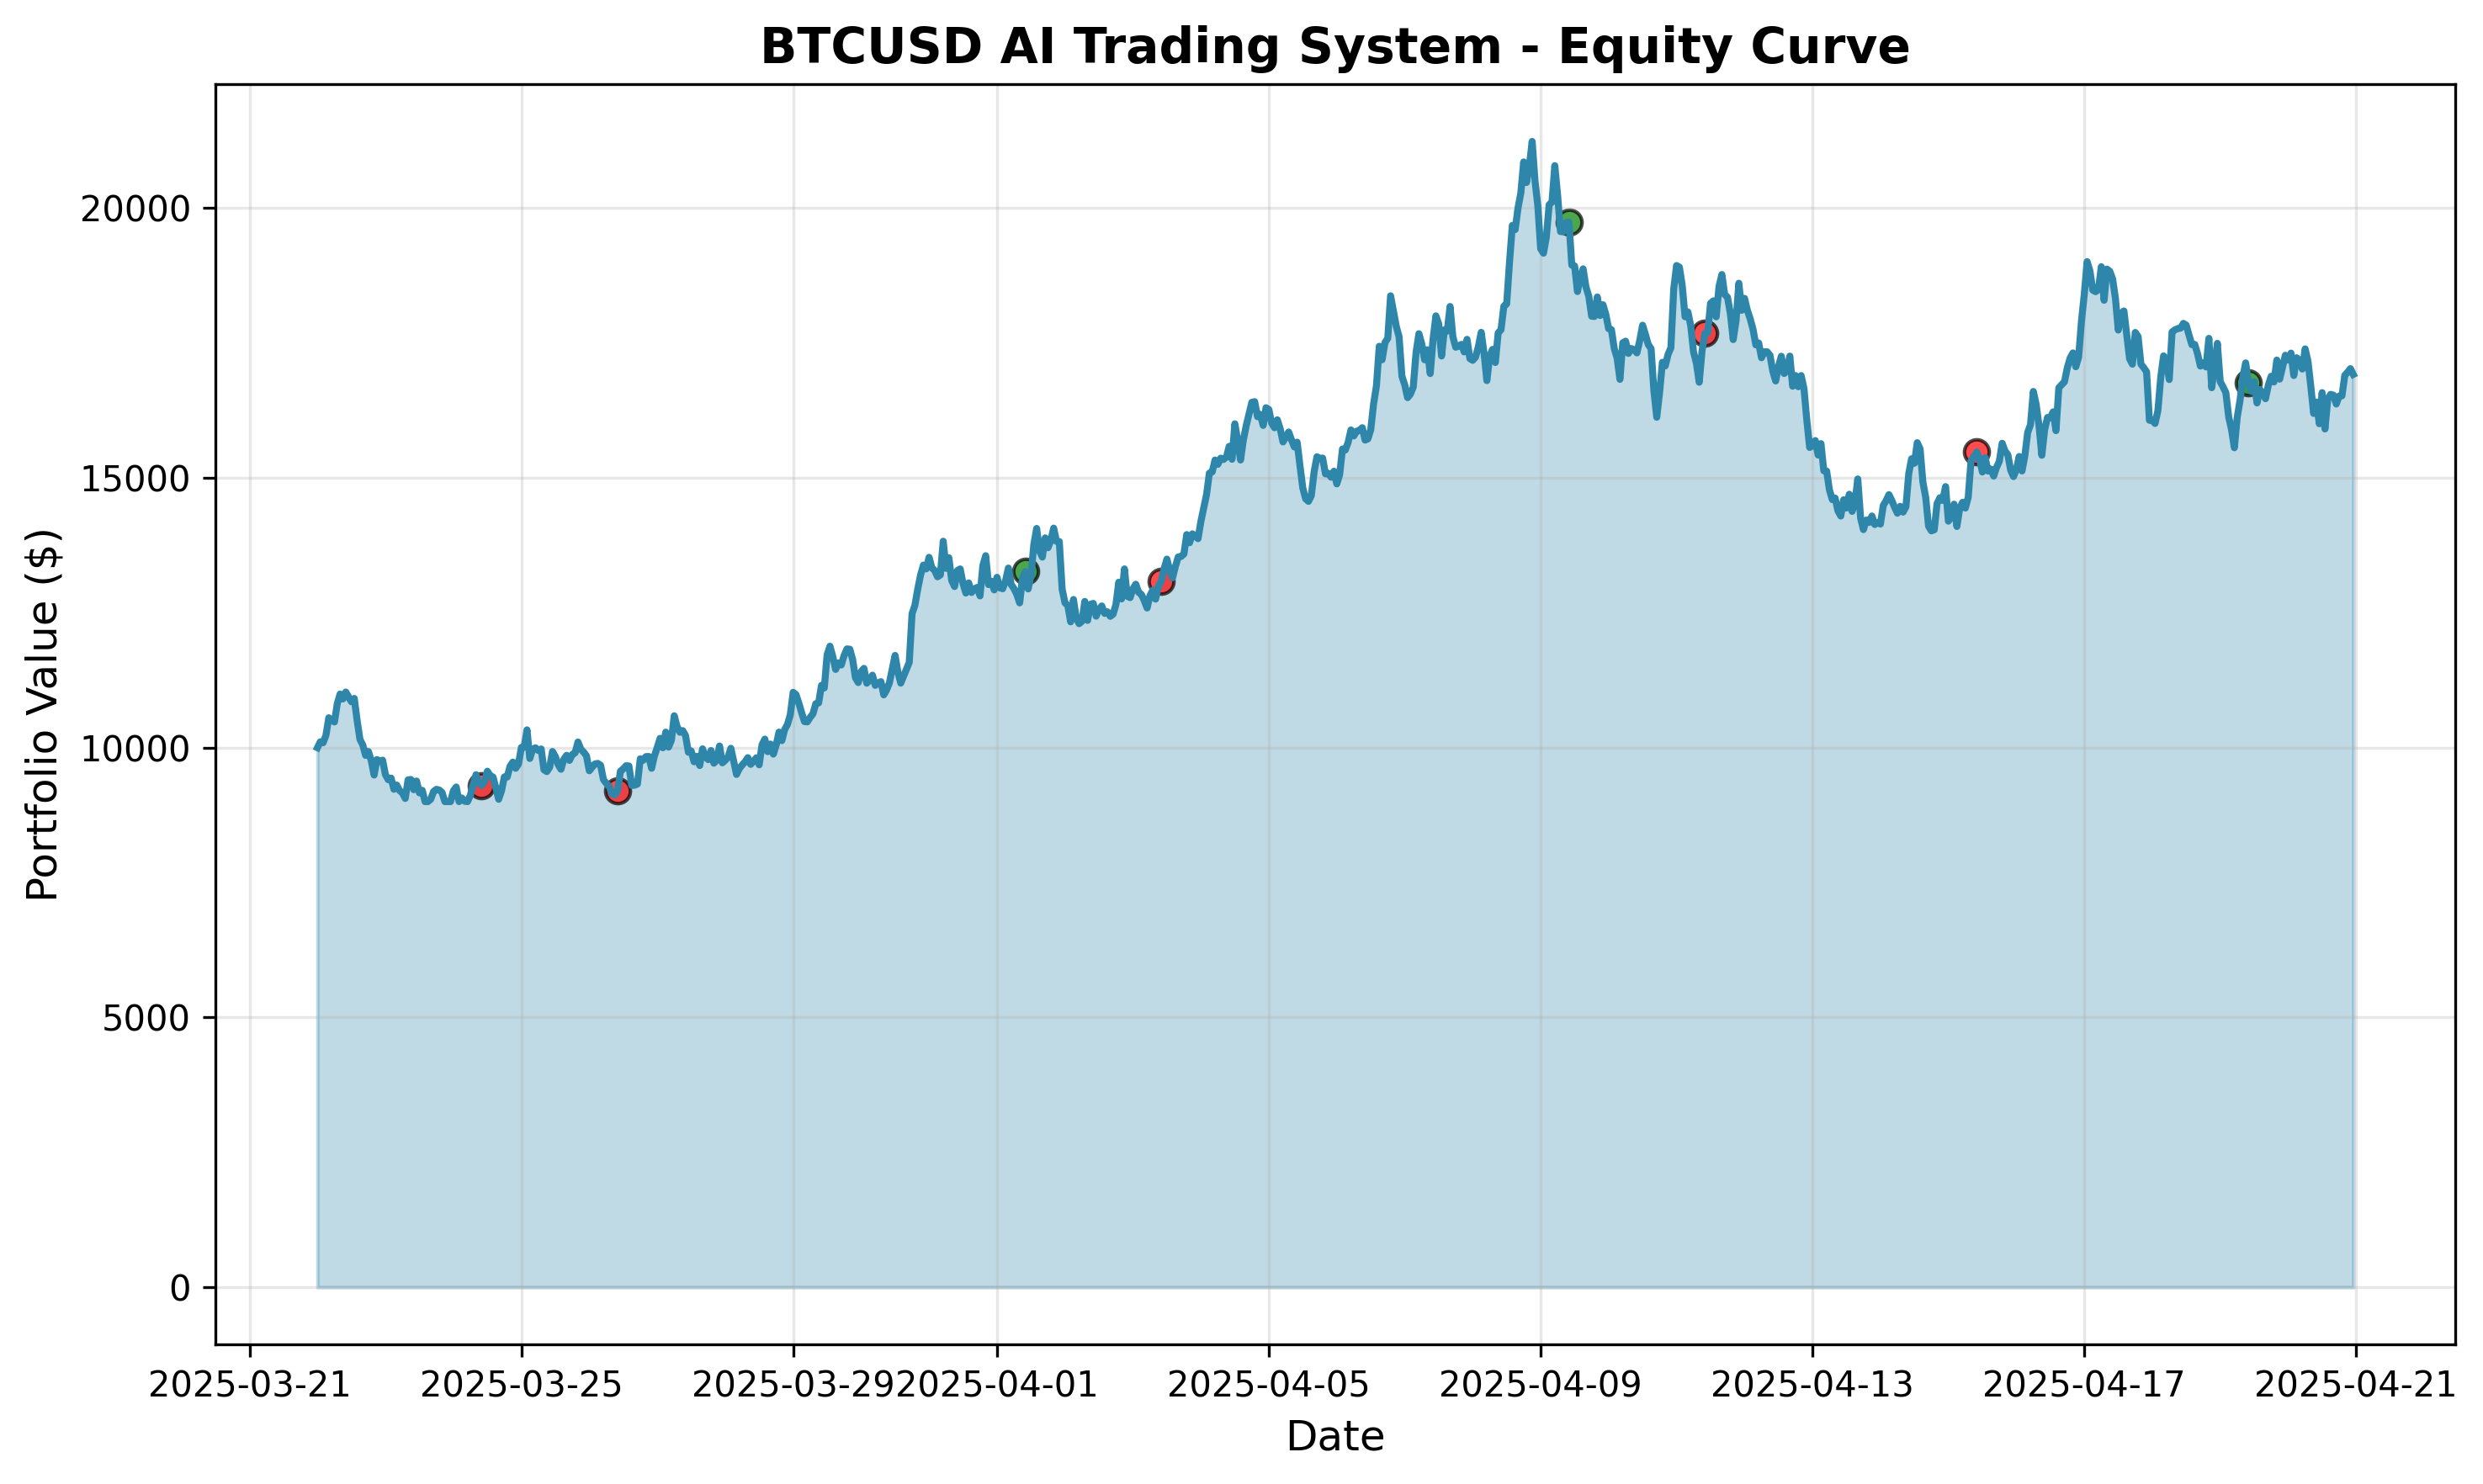
\includegraphics[width=0.9\textwidth]{figures/equity_curve.png}
    \caption{Simulated equity curve showing portfolio value over the backtesting period. Green/red markers indicate profitable/loss-making trades.}
    \label{fig:equity}
\end{figure}

\begin{figure}[ht]
    \centering
    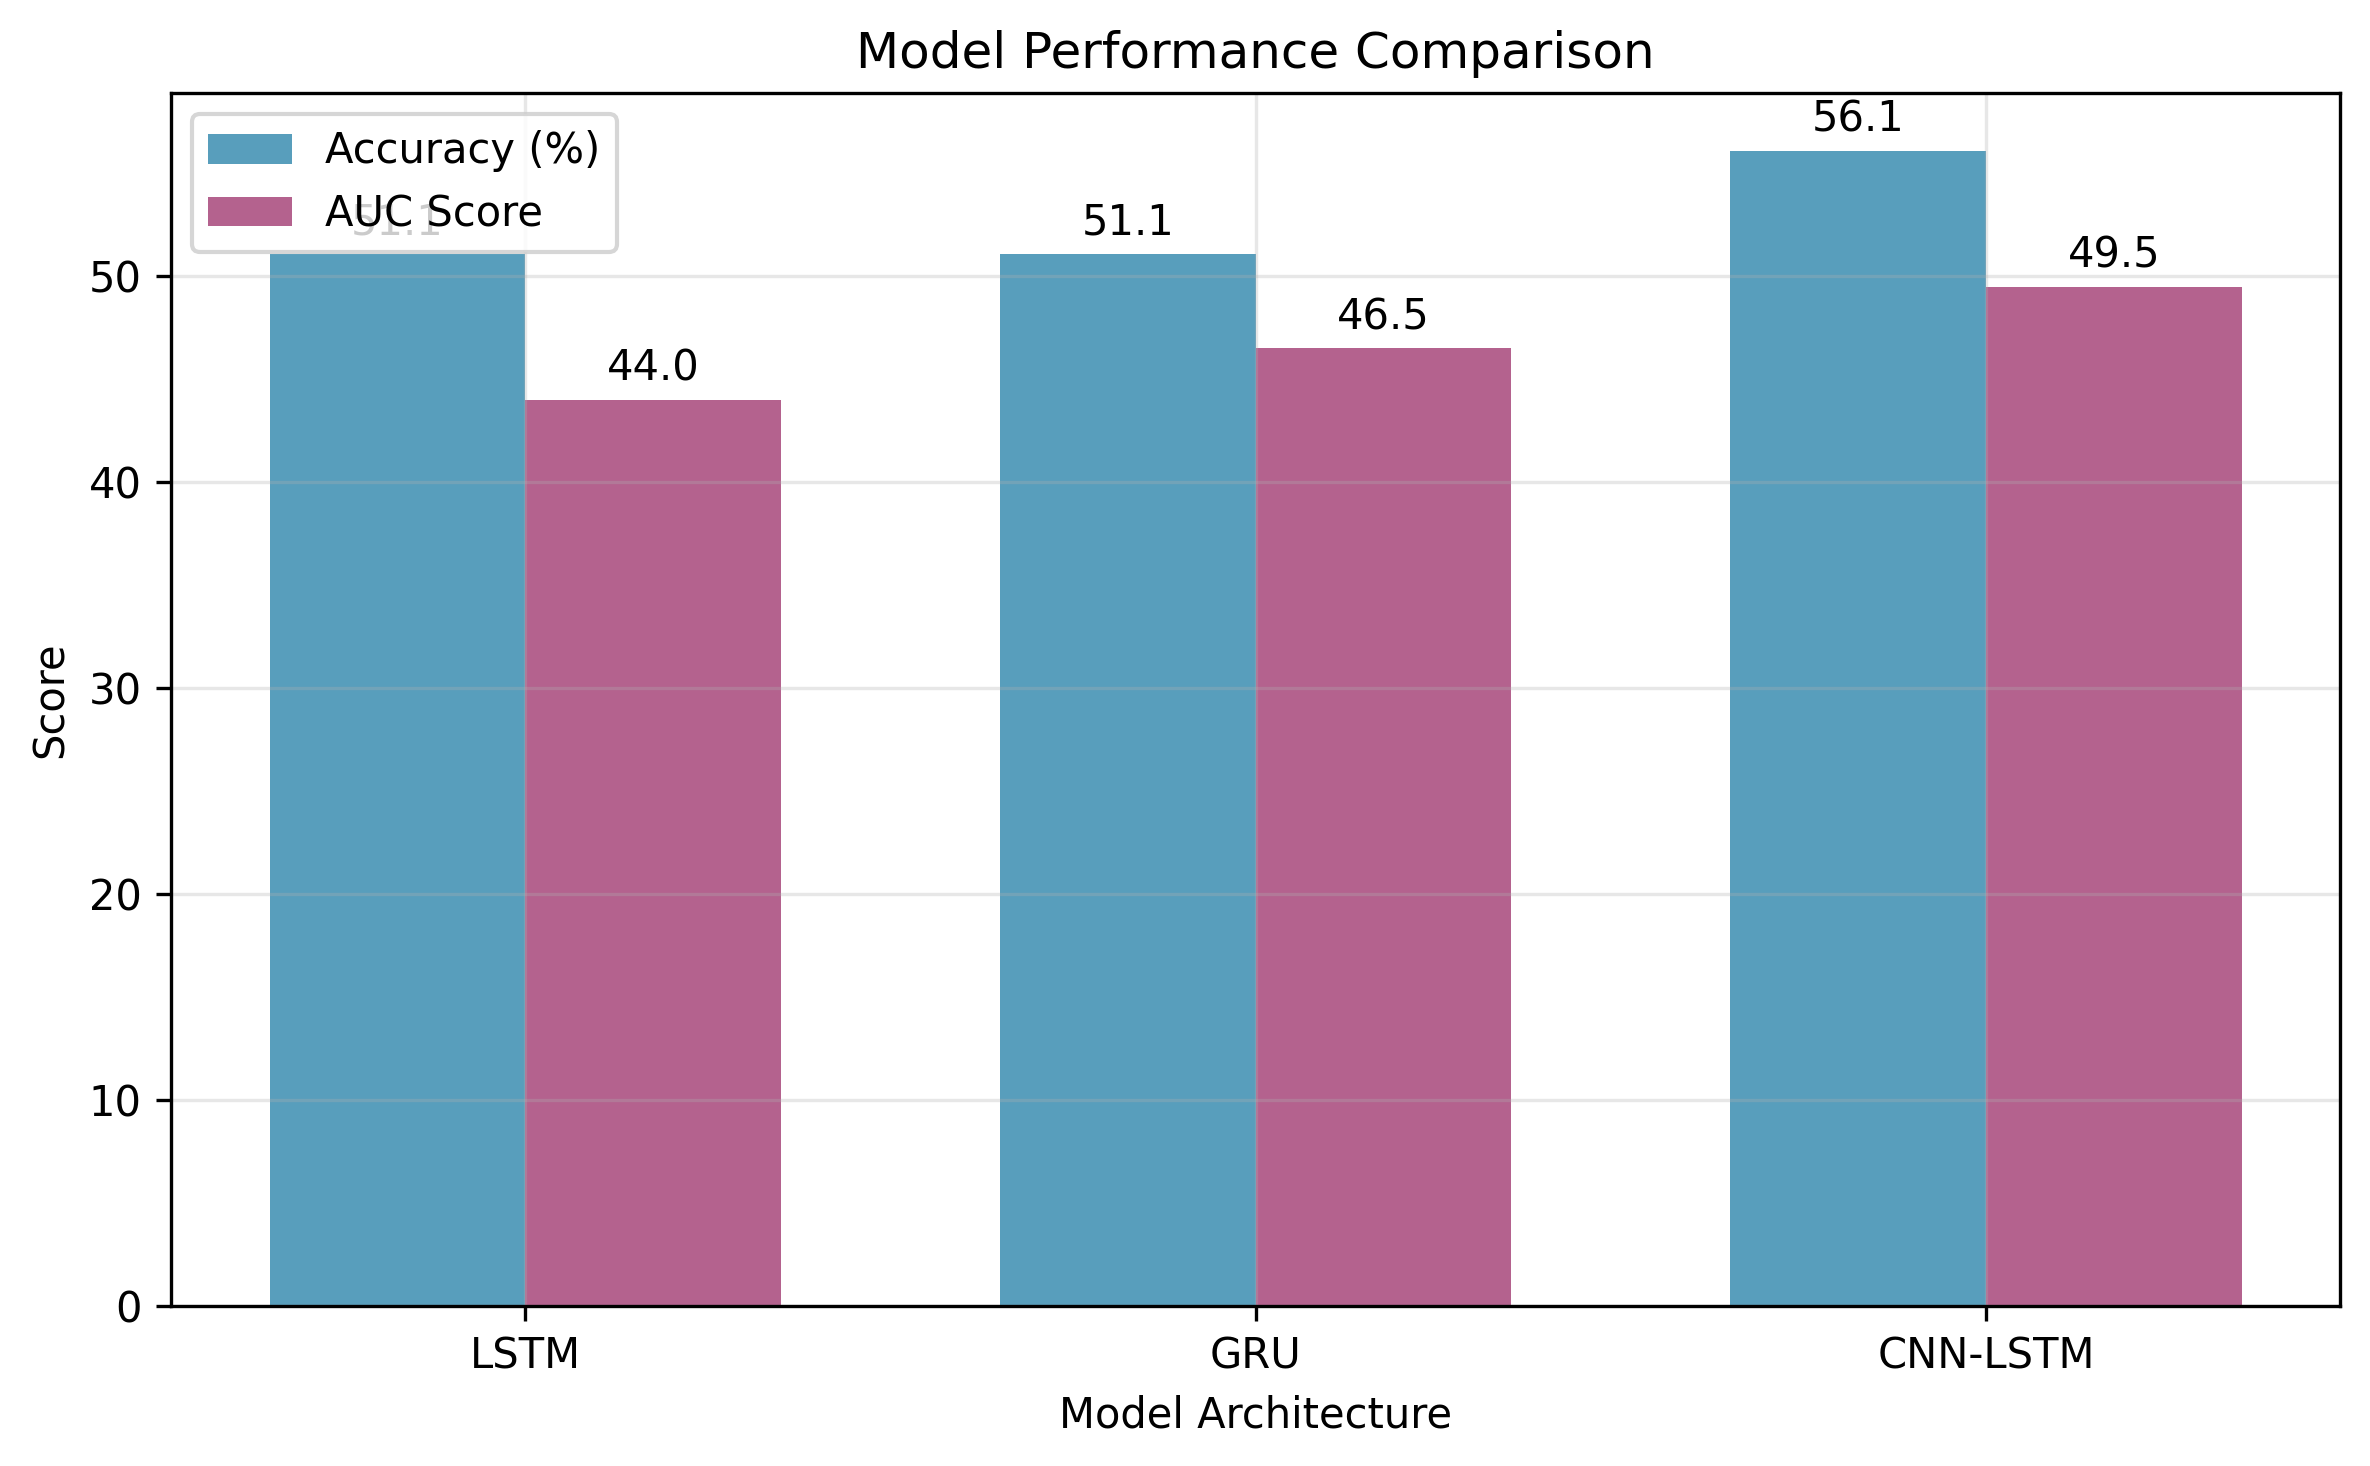
\includegraphics[width=0.8\textwidth]{figures/model_comparison.png}
    \caption{Comparison of individual model performance metrics across architectures.}
    \label{fig:model_comparison}
\end{figure}

\section{Deployment and Live Trading}
We detail practical considerations for production deployment: model retraining cadence, feature pipeline monitoring, data quality checks, safety limits (daily exposure cap, max position size), and paper trading before live funds. The repository includes a \texttt{train\_and\_trade.py} orchestrator and a \texttt{live\_trading} module with paper trading mode.

\section{Limitations and Future Work}
Limitations include non-stationarity, potential overfitting to market regimes, and data source reliability. Future work includes dynamic model weighting, more extensive hyperparameter search, and multi-horizon prediction models.

\section{Conclusion}
We present an end-to-end ensemble approach to short-term BTCUSD prediction and trading, with modular training, backtesting, and deployment components. The included codebase supports reproduction and further experimentation.

\section*{Acknowledgments}
Thanks to the open-source libraries and community for tooling and research that made this work possible.

\bibliographystyle{plain}
\bibliography{references}

\end{document}
